
\section{Design}

We had two major challenges: to speed up the algorithm and to make BP converge when it has multiple optima.

\subsection{Dataset}
Two different datasets are used. 

\textbf{Random dataset} is generated randomly with 1\% of all possible edges.

Edge weight are set to the integers between 1 and $\frac{|S| * |U|}{100}$ if S is one subset of nodes U is the other subset.

\textbf{Realistic dataset} is from "The University of Florida Sparse Matrix Collection~\cite{sparseMatrix}".
The distribution of edge weights are mostly biased.

We first tested our implementation with random dataset then moved on to the realistic dataset.

\subsection{Initialization}
For speedup, we initialized messages with respect to edge weights.
The larger the weight, the more likely the edge to be selected. 
Therefore, by assigning proper initial values, it is possible to accelerate convergence.
Figure~\ref{fig:init} shows the relationship between convergence time and initialization coefficient.
The convergence was fastest when the initial messages were set to the half of the edge weights.
\begin{figure}
\centering
%\includegraphcs[width=1.0\columnwidth]{system.pdf}
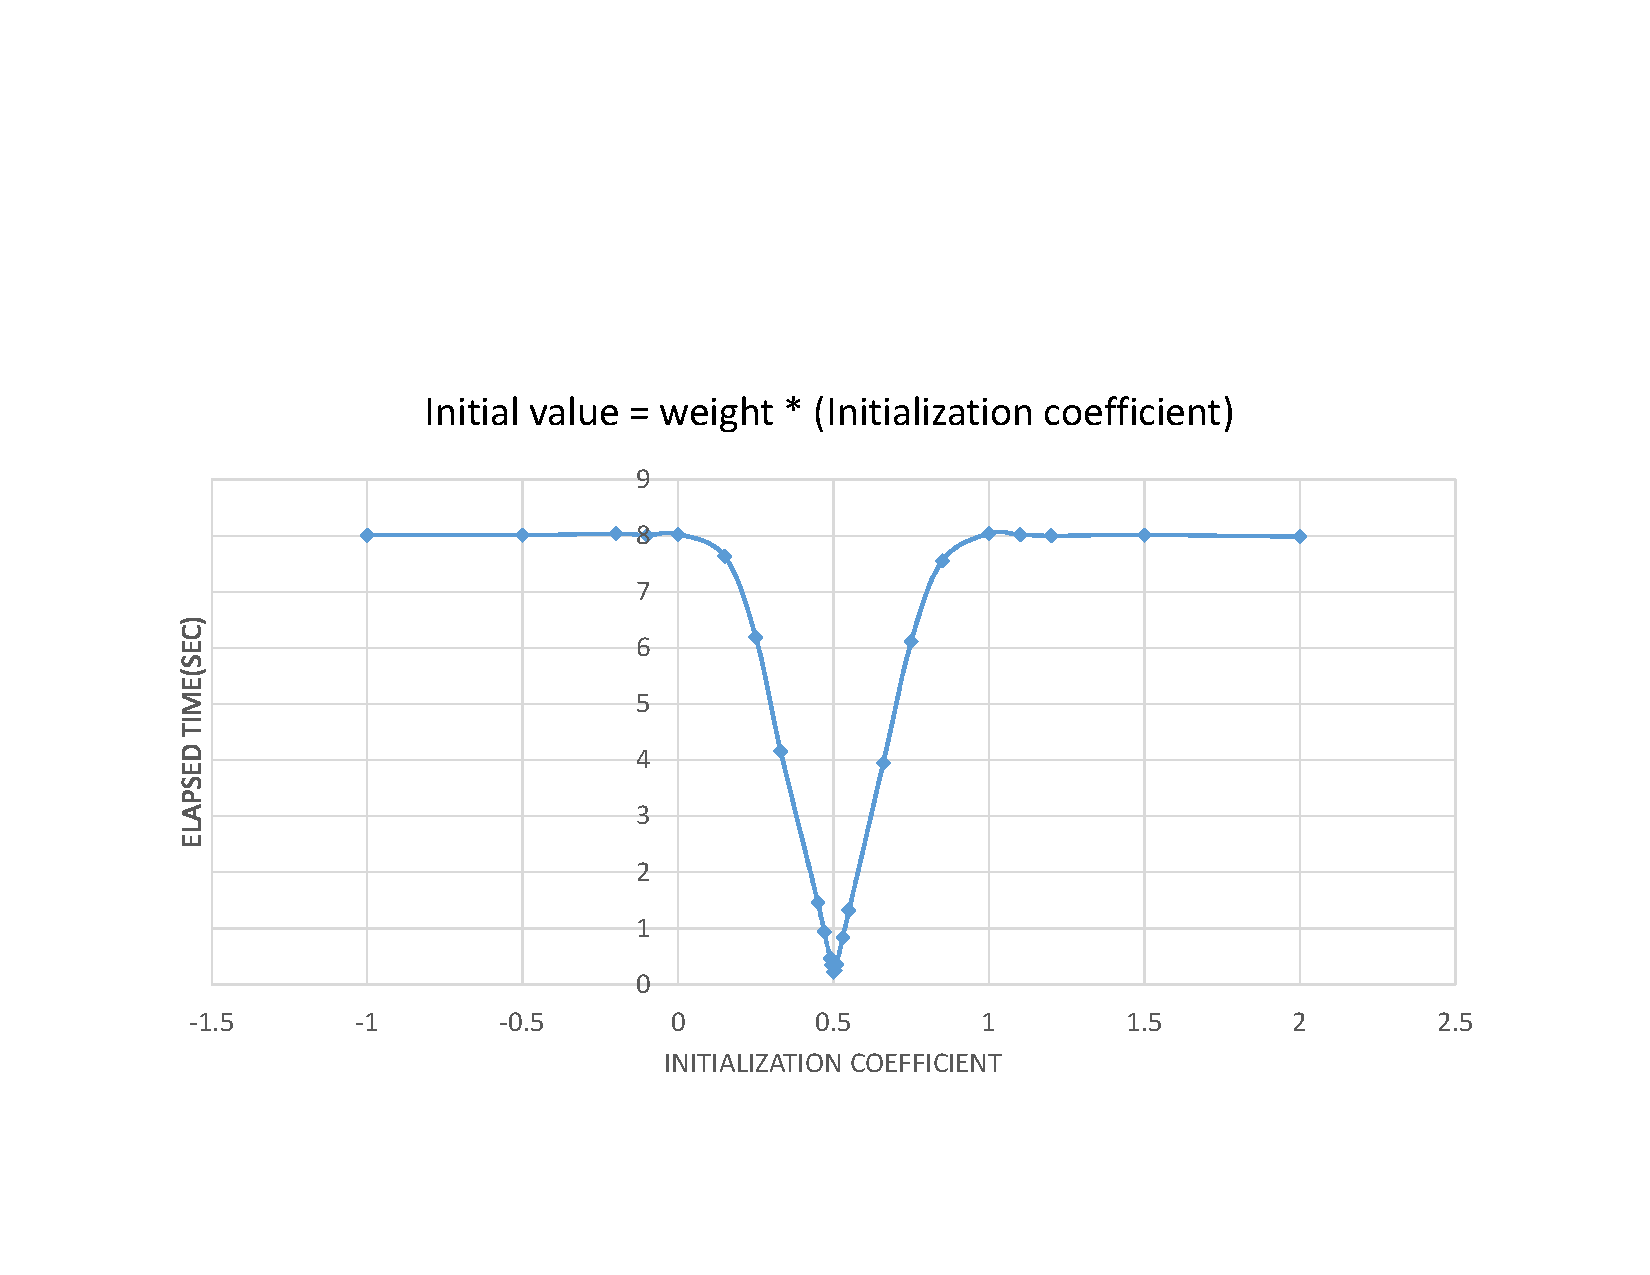
\psfig{file=init.pdf, height=1.5in, width=3in}
\caption{Convergence time gets shorter as the coefficient gets closer to 0.5}
%\tightcaption{aaaa}
\label{fig:init}
\end{figure}

\subsection{Noise}
The algorithm converges only when it doesn't have any fractional optima. 
However, sometimes the data has multiple optima, especially the realistic data. Biased weight distribution leads to a lot of fractional optima. 

To enforce convergence by making the solution unique, we added a weight noise to the current weight and removed it after convergence. 
This method would not affect to the solution only if the sum of all the noises is less than 1. 

To avoid each noise being too small, the noise was only added to \textbf{unstable edges}, the edges that the decision keeps changing after several iterations. 
Here, the noise was given after first 100 iterations and the edges were marked unstable after 20 iterations. 

\begin{figure}
\centering
%\includegraphcs[width=1.0\columnwidth]{system.pdf}
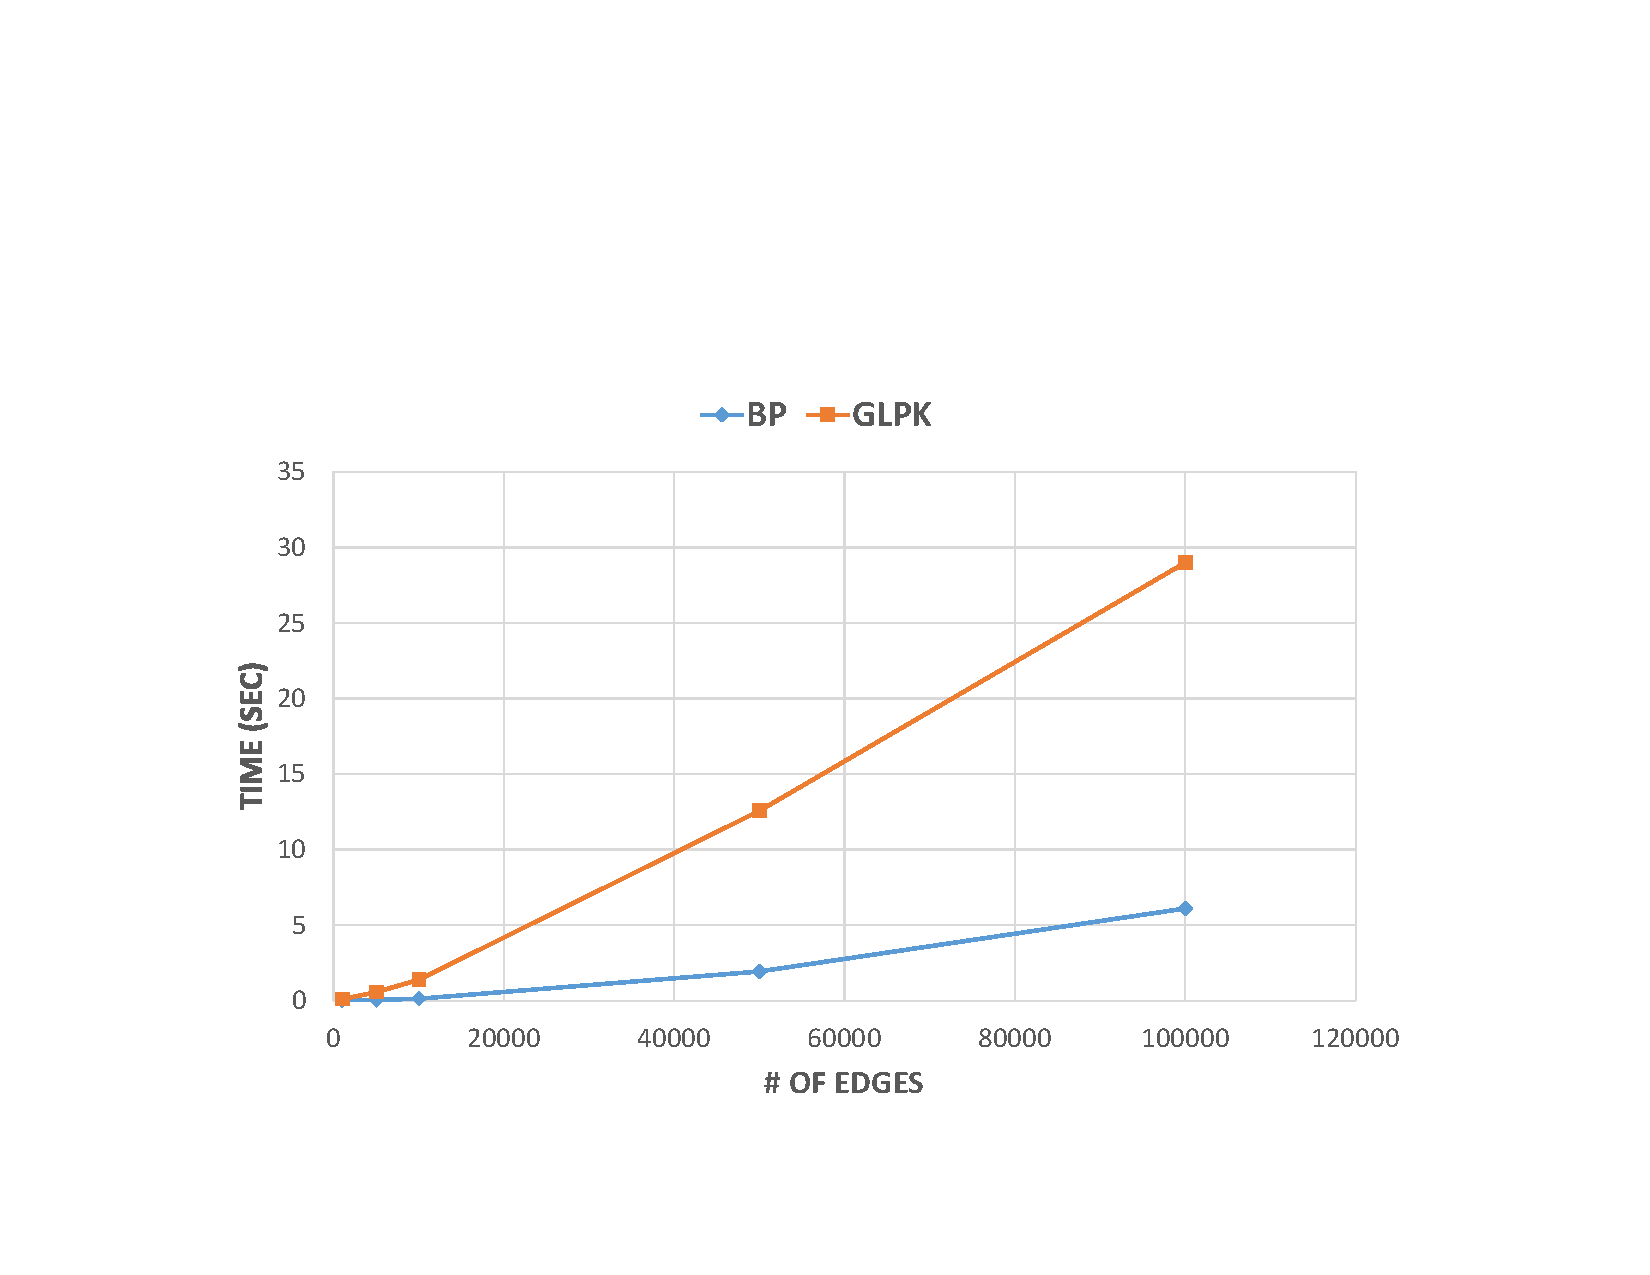
\psfig{file=randomconv.pdf, height=1.5in, width=3in}
\caption{Convergence time of random dataset}
%\tightcaption{aaaa}.
\label{fig:randomconv}
\end{figure}

Let n the number of unstable edges. The noise is a random number between 0 and 1/(n+1). 

Figure~\ref{fig:randomconv} shows the convergence time of random dataset when the noise was given after 100 iterations. BP was up to 12.54 times faster than GLPK.

Realistic dataset has much more fractional optima then the random dataset. Most of the random dataset reached convergence after giving random noise once, however, the realistic dataset barely did. We tried adding another noise and run after removing previous noise until convergence. The noise was added after every 100 iterations.

\begin{figure}
\centering
%\includegraphcs[width=1.0\columnwidth]{system.pdf}
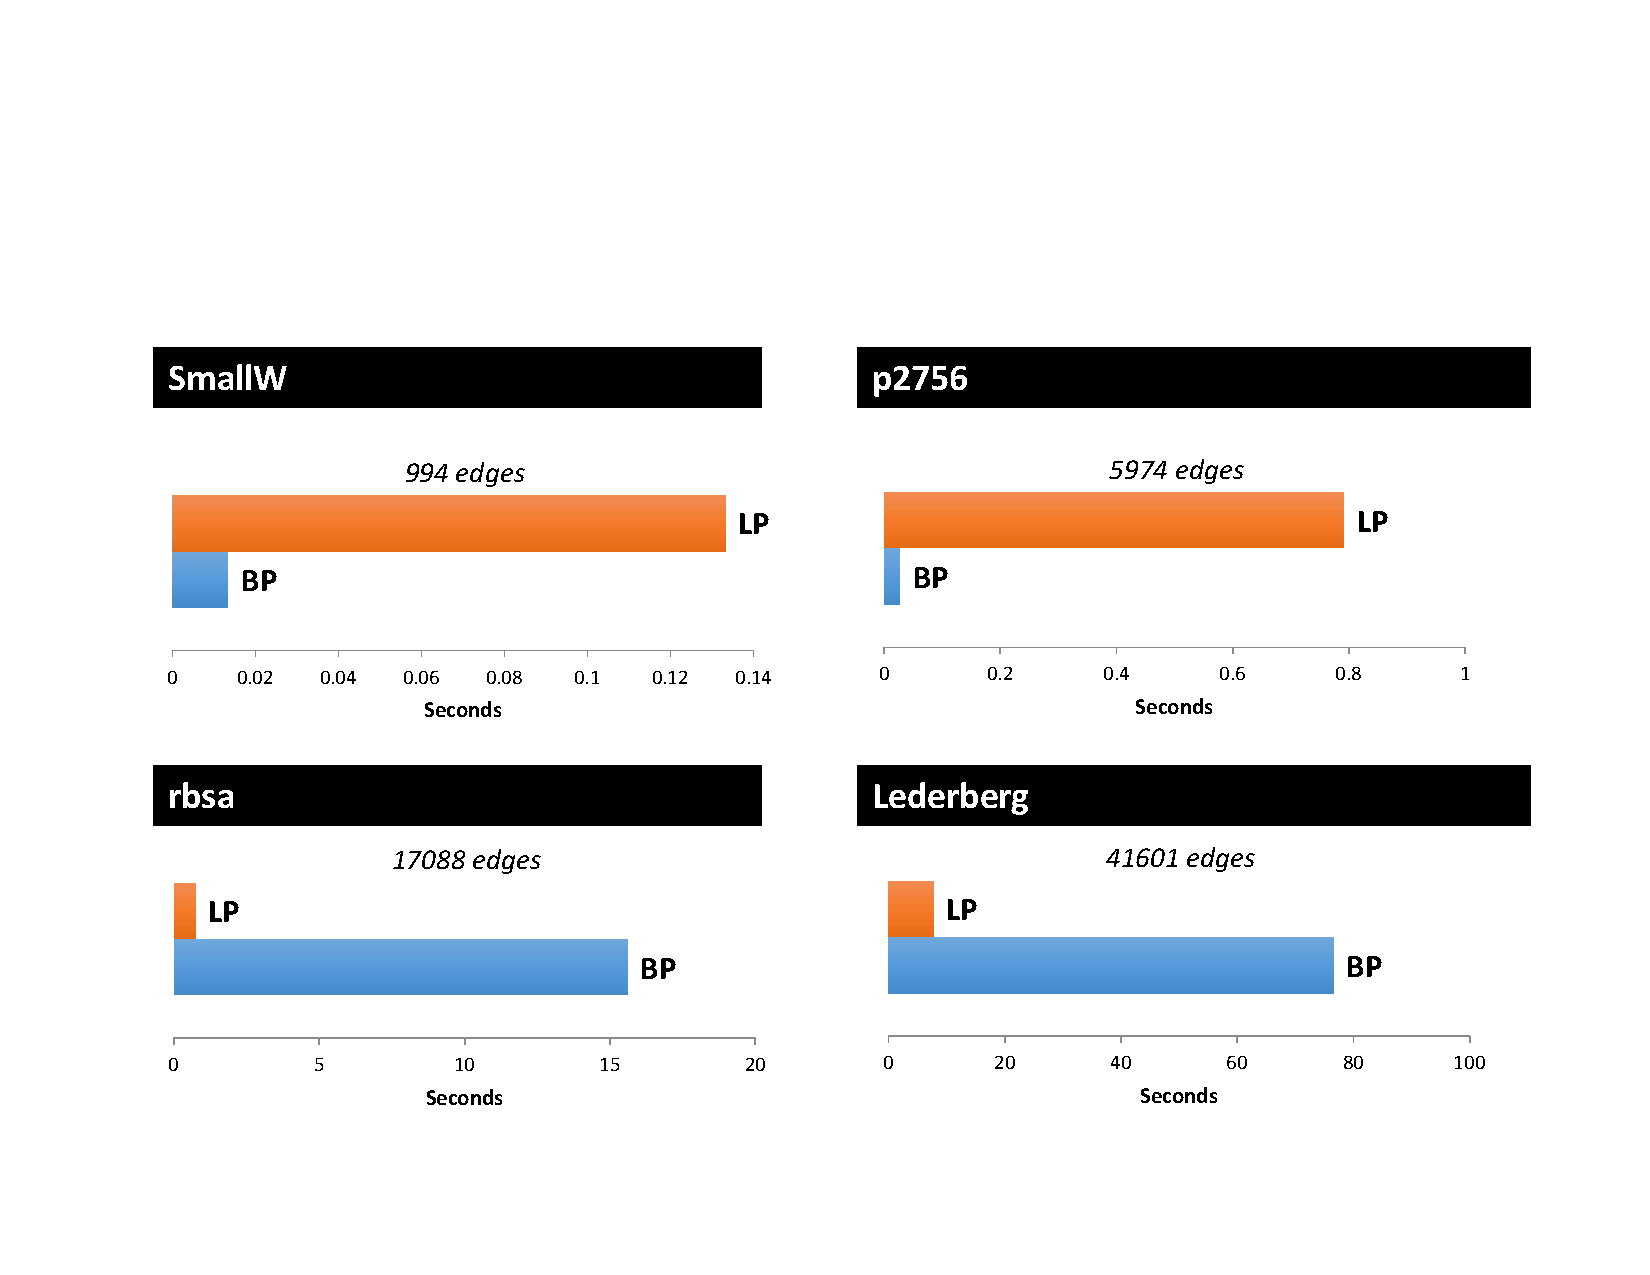
\psfig{file=realisticconv.pdf, height=1.5in, width=3in}
\caption{Convergence time of realistic dataset}
%\tightcaption{aaaa}
\label{fig:init}
\end{figure}

The result varies with the input data. Since GLPK is multi threaded, the performance of BP is still comparable to that of LP.

However, repeating the same step is inefficient until it gets the best noise by generating random noise sets. 
In figure~\ref{fig:sum_v_iter}, we enforced matching after every 100 iterations before adding noise and plotted current weight sum with respect to the number of iterations. 
An edge is randomly selected when a node is connected to multiple edges.
The result shows that BP gets near optimum quickly and there is not much difference after once the noise is given. 

\begin{figure}
\centering
%\includegraphcs[width=1.0\columnwidth]{system.pdf}
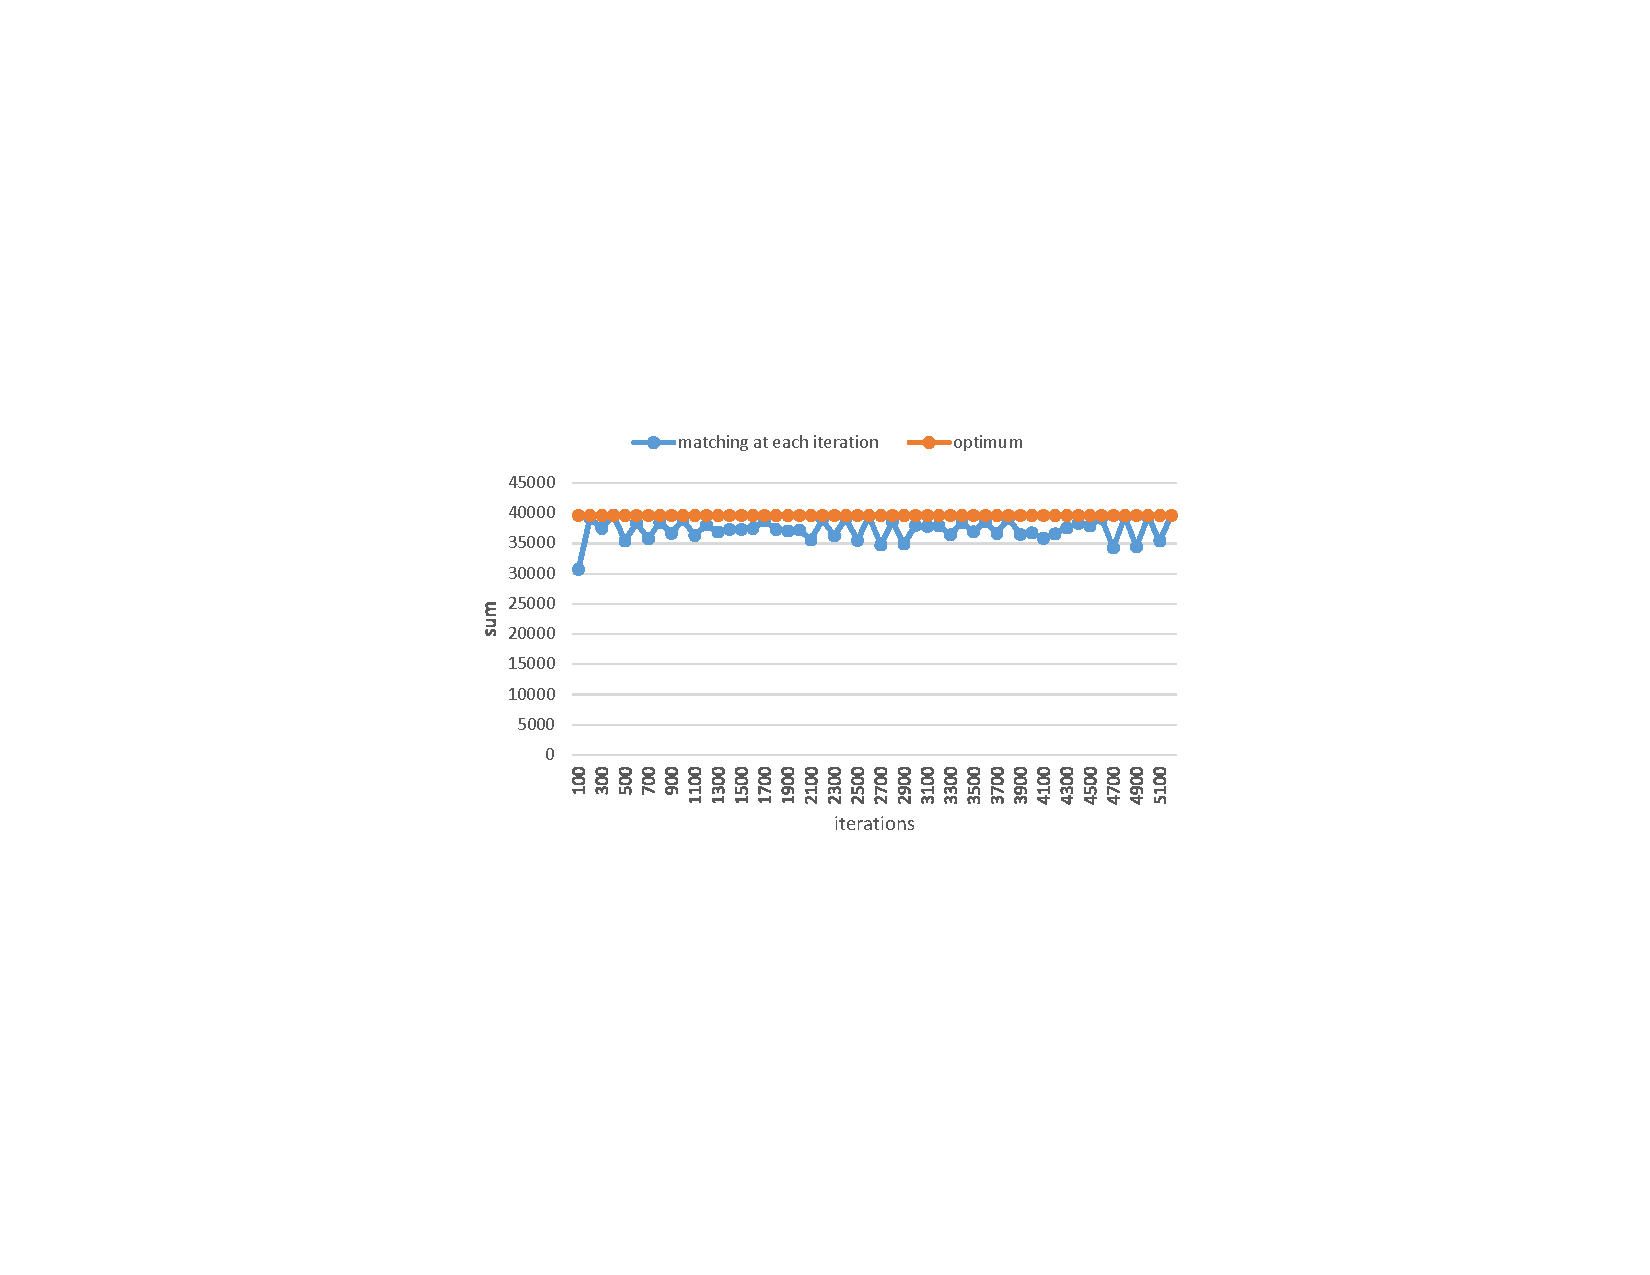
\psfig{file=sum_v_iter.pdf, height=1.5in, width=2.5in}
\caption{Weight sum of current matching stays near optimum}
%\tightcaption{aaaa}
\label{fig:sum_v_iter}
\end{figure}

\subsection{Multi-threading}
Using the fact that BP is a graph-parallel algorithm, a multithreaded algorithm can be devised. Two methods were explored: synchronous and asynchronous. The single-threaded version of the algorithm sequentially updates the belief messages for each node and then sequentially passes the messages through via the edges, which is considered to be one iteration of the algorithm. The general concept of the single-threaded version is to prepare the messages then pass them when all nodes have prepared their messages. 

In the synchronous multithreaded version, the algorithm tries to mimic this behavior but to reduce the computation time by dividing up the graph and doing iterations concurrently, while also synchronizing the start of message preparation and delivery. First, the graph is divided up into groups with equal number of nodes and edges. Then, for each iteration, a group is assigned to a thread to prepare their messages and pass them. The threads must synchronize between each iteration and also between the message preparation stage and the passing stage to ensure that all nodes have prepared their messages before passing them.

In the asynchronous version, however, the idea of an iteration is slightly loosened. The synchronization step in between the preparation and passing stage is discarded and multiple iterations are done at once. Instead of having to wait for each iteration to start, the threads continually prepares and passes messages until they are stopped by the main process or until the algorithm converges.

The performance of each algorithm was tested by testing multiple randomly generated bipartite graphs of varying sizes and configurations. Five different graph node sizes were chosen for which five different graphs with different connection configurations were tested twenty times each. The performance was measured by time alone, but the number of iterations was also recorded for further analysis.

\subsubsection{Synchronous}
Three functions were added to the single-threaded version of the BP solver. Two functions were newly added - the makeThread and processThread function - and a preexisting function was modified - the oneIteration function. 

The makeThread function makes multiple slave threads, each one running the processThread function, and returns when they are ready. It is this function that randomly divides up the graph into groups and assigns it to each slave thread. It also assigns the necessary shared variable addresses between the threads and the condition variables to wait on. This function must be called before the main BP solver loop to initialize the slave threads.

The oneIteration function is modified to wake the slave threads for one iteration of the BP algorithm. It waits for the slave threads to signal the end of their iteration and then returns.
The processThread function is the designated method for each thread. One the thread is initialized, it updates the number of threads ready and waits on the wakeup condition specified by the makeThread function. If the desired number of threads are made - 12 in our implementation - then the last thread to go into the waiting state signals the main thread of the initialization before going into its dormant state. The slave threads are only woken up by the oneIteration function signaling for the thread wakeup and iterate procedure. The slave threads first prepare the node messages for their assigned node groups and then wait for all the threads to finish. Once all the threads have finished preparing their messages, they start passing the messages to their respective edges of their assigned groups. Once the threads all finish, the last thread to finish signals the main thread of the job completion and all the threads wait to be woken up again.

\begin{figure}
\centering
%\includegraphcs[width=1.0\columnwidth]{system.pdf}
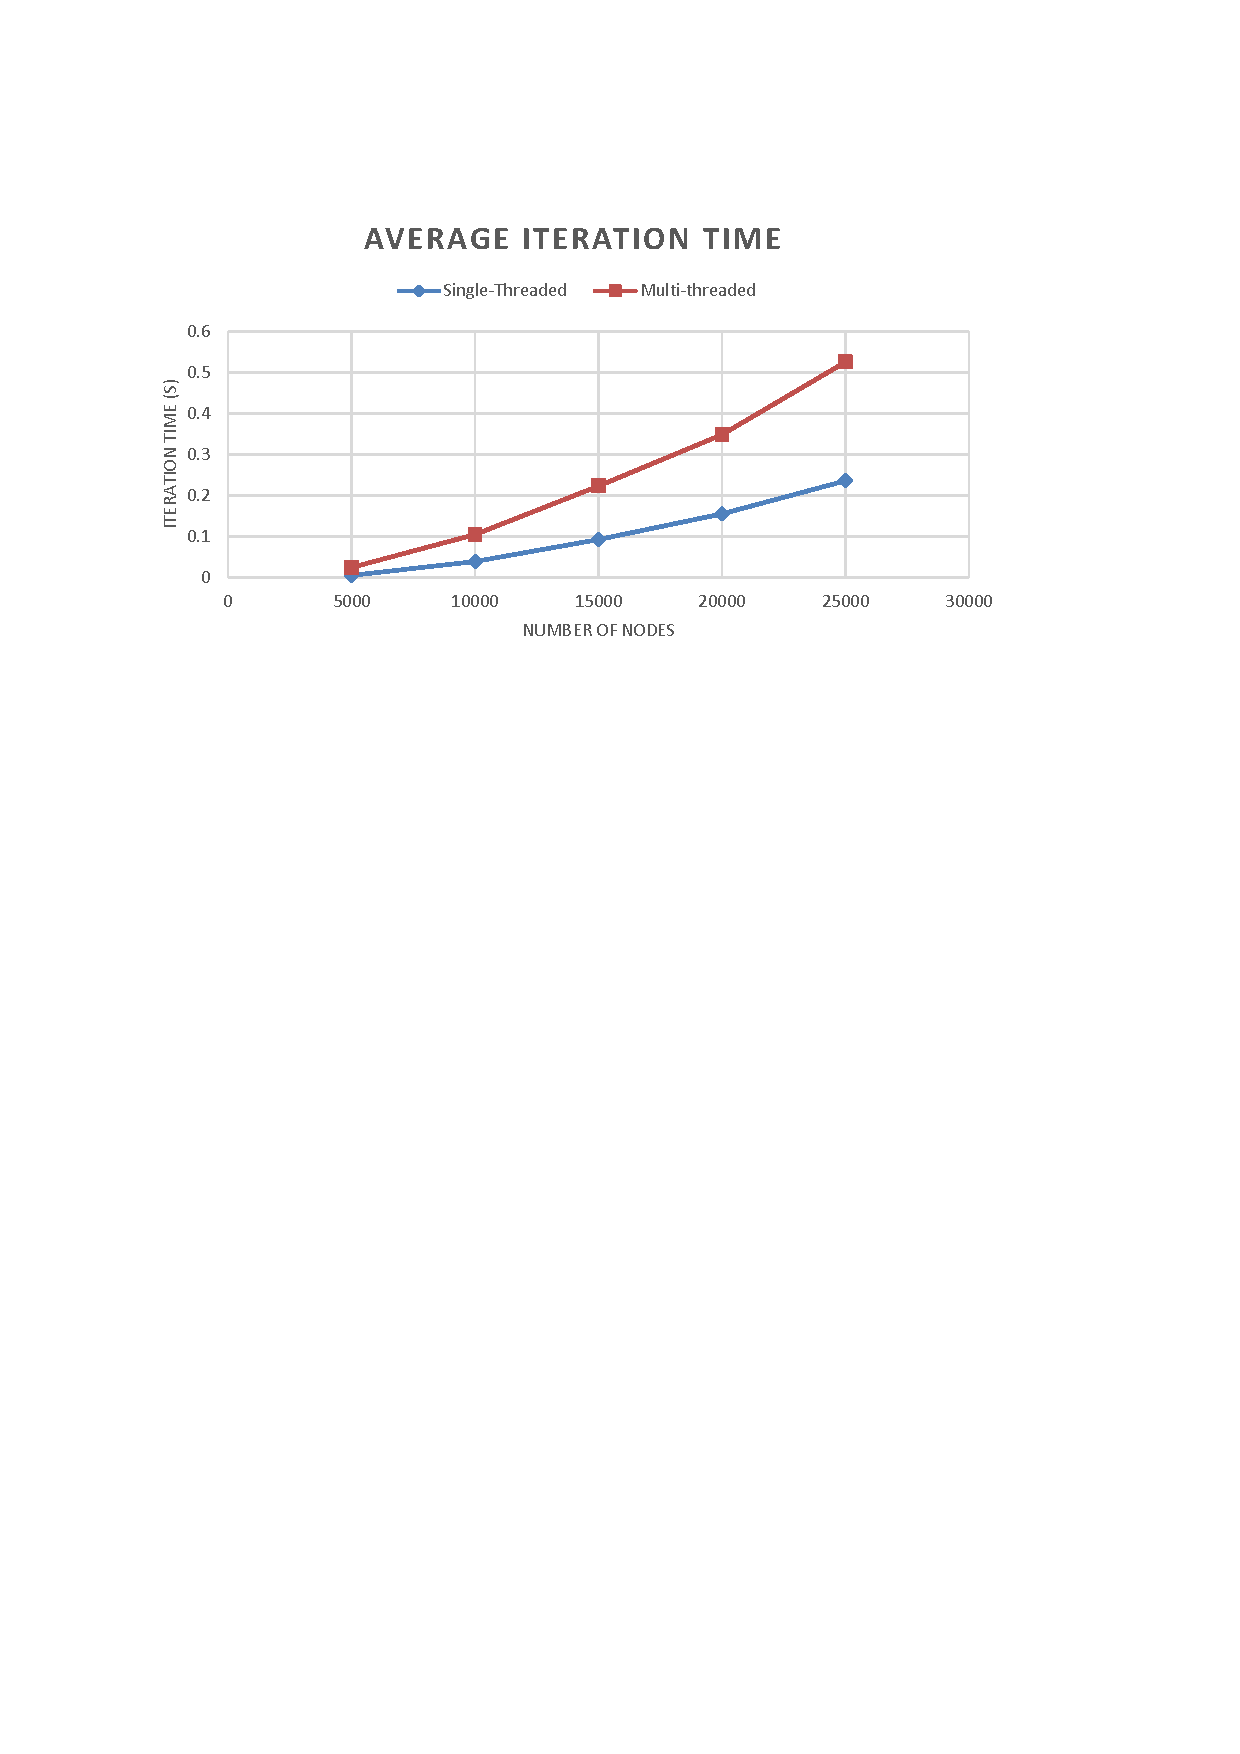
\psfig{file=bd1.pdf, height=1.5in, width=3in}
\caption{Weight sum of current matching stays near optimum}
%\tightcaption{aaaa}
\label{fig:bd1}
\end{figure}
As figure~\ref{fig:bd1} shows, the average time for the synchronous algorithm is higher than that of the single-threaded version. The most likely explanation for this is the additional overhead time for the multithreaded version's framework. The main thread has to wake each slave thread individually and each slave thread has to wait for other threads to finish their work for it to move on. These small inconveniences add may add up to a huge bottleneck.

To further investigate the source of the long runtime, we plotted the average time it takes per iteration, as follows:
\begin{figure}
\centering
%\includegraphcs[width=1.0\columnwidth]{system.pdf}
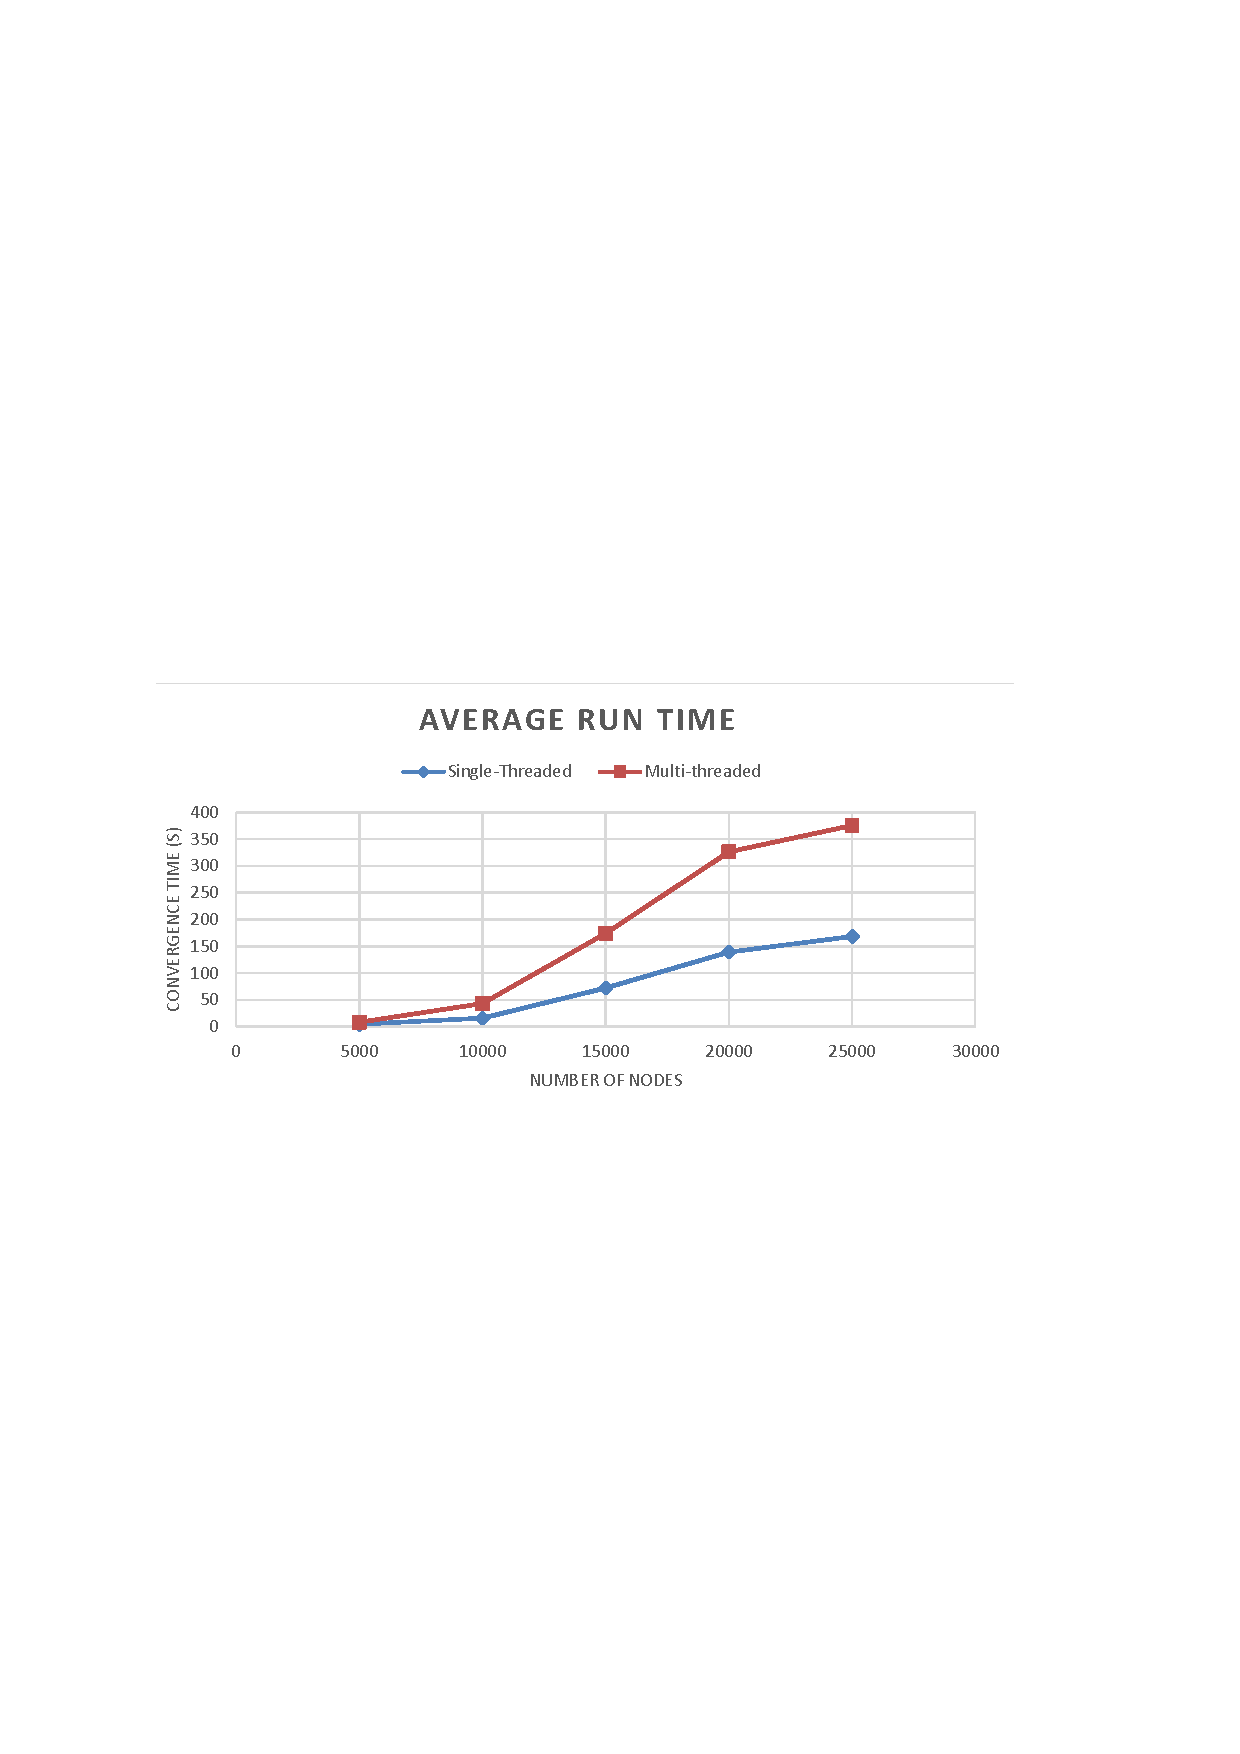
\psfig{file=bd2.pdf, height=1.5in, width=3in}
\caption{Weight sum of current matching stays near optimum}
%\tightcaption{aaaa}
\label{fig:bd2}
\end{figure}

Figure~\ref{fig:bd2} suggests that the wait time between slave threads to finish is causing more of the time delay than the wake-up procedure, as the wake-up should only make a constant time difference for each iteration.

\subsubsection{asynchronous}
In the asynchronous version, the three functions in from the synchronous version are modified and another new function is added - the Iterate function.

The makeThread function is kept the same except for the shared variables it must additionally assign to each slave thread.
The oneIteration function is reverted back to its single-threaded algorithm. This is only used to check whether the algorithm has converged or not in an incremental fashion, as the main function that handles iterations does multiple iterations at once, making it inconvenient for convergence checking.

The Iteration function works similar to the oneIteration function from the synchronous version, but it takes in an extra integer as an input. This integer value determines how many iterations the algorithm will approximately iterate before returning. This number is set to 20 in our implementation.

The processThread function works quite similarly to that of the synchronous version with some changes. One difference is that this version does not wait in between the message preparation and passing phases of the algorithm, they simply keep iterating through them without waiting until they reach a certain number of iterations. Another difference is that the slave threads do multiple iterations, instead of one, to signal the master thread to notify that they are done. The makeThread function randomly designates one of the slave threads as the counter that counts the amount of iterations it has done. When the counter thread reaches the desired number of iterations, it signals all the other slave threads to stop and wait after finishing their current iteration, regardless of how many iterations they have done. Then, when the slave threads all finish, they wait to be woken up again and signal the master thread that the job is done.

When testing a graph with 5000 nodes and 62500 edges, the algorithm converged after 57088 iterations and spent 523.820 seconds, which is 60 times the average iteration and a hundredfold the time it took for the single-threaded version. We speculate that the main problem lies in the data race of the nodes and the edges, as an edge might be stuck with a stale value for a long time until it is updated in the asynchronous version. This also explains why the algorithm fails to converge at times.

